\chapter{Results}
The systems works quite well within most of the requirements from specification although not all specifications have been completely fulfilled. The precision is not within 5 cm but rather 10 cm, but this could have easily been calibrated. The system updated around 12 times a second which is somewhat real time. This could have also been improved but wasn't really necessary.\\
The final result is shown on figure~\ref{fig:totalsys}. A graphical presentation of our results is shown in table~\ref{table:alltest}
\begin{figure}[hbpt]
\centering
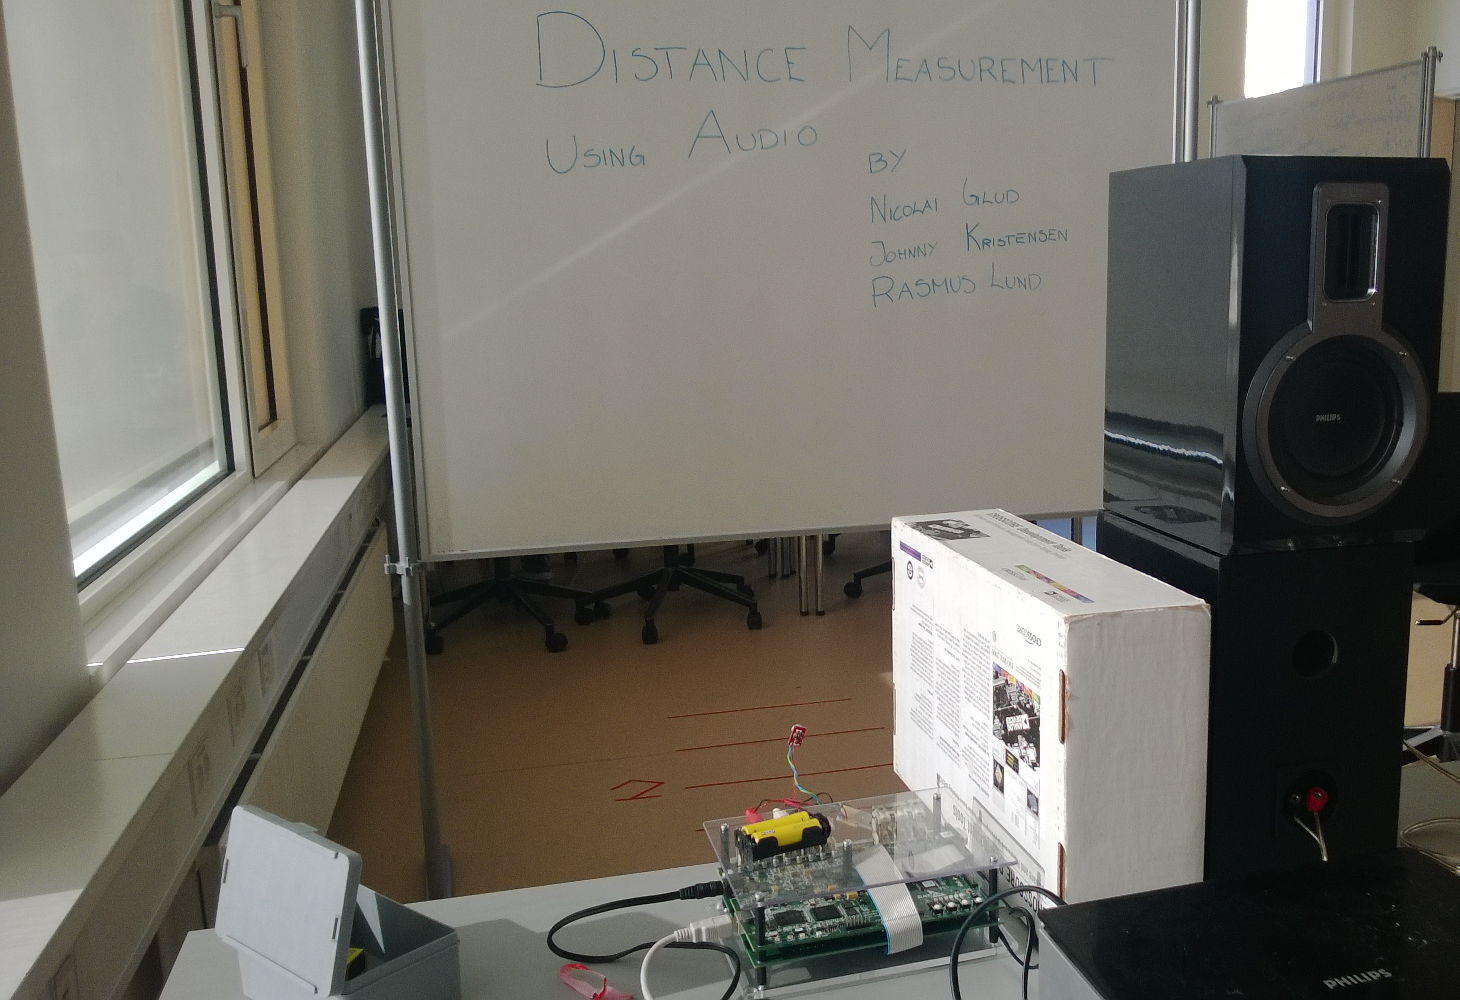
\includegraphics[scale=0.2]{billeder/totalsys}
\caption{Total system}
\label{fig:totalsys}
\end{figure}

\begin{table}[H]
\centering
\begin{tabular}{c c c c}
\hline
Approved & Approved with comment & Not approved & Not tested \\
$\surd$ & $\times$ & $\div$ & $\diamond$ \\\hline
\end{tabular}
\caption{Test Approval Categories}
\end{table}

\begin{table}[H]
\centering
\begin{tabular}{ c c c }
\hline
Requirement: & Status & Comment \\ \hline
Use of DSP & $\surd$ \\
Sound output & $\surd$ \\
Sound input & $\surd$ \\
Precision: <5 cm & $\times$ & <10 cm which is acceptable for now \\
Range: 25cm - 250 cm & $\surd$ \\
Frequency band: 14 - 16 kHz & $\surd$ \\
Memory: max 32kB & $\surd$ \\
System must be real-time & $\times$ & Acceptable for now \\ \hline
\end{tabular}
\caption{Requirement results}
\label{table:alltest}
\end{table}

\chapter{Improvements}
This chapter contains thoughs about the improvements we want to make to our system but did not have the time to do.
\section{Using the system as an actual musical instrument}
\subsection{Playing notes}
The system outputs a sine wave sound. This is great for demonstrative purposes but might not be as pleasant to listen to. What makes a musical sound or "note" pleasant to listen to is harmonics. Most musical tones are composed of fundamental tone and multiple overtones. A sequence of a fundamental tone and 3 overtones would then consist of 4 harmonics. Mathematically, tones are composed of the fundamental frequency and multiples of fundamental frequency like so:\\
\begin{itemize}
\item 1 * freq : fundamental tone : 1st harmonic
\item 2 * freq : 1st overtone     : 2nd harmonic
\item 3 * freq : 2nd overtone     : 3rd harmonic
\item n * freq : (n-1) overtone   : nth harmonic
\end{itemize}
This is also shows on figure ~\ref{fig:harmonics}. To produce such a signal on an embedded unit we would have to use the principle of Fourier series and add the different frequency components together. 
\begin{figure}[hbpt]
\centering
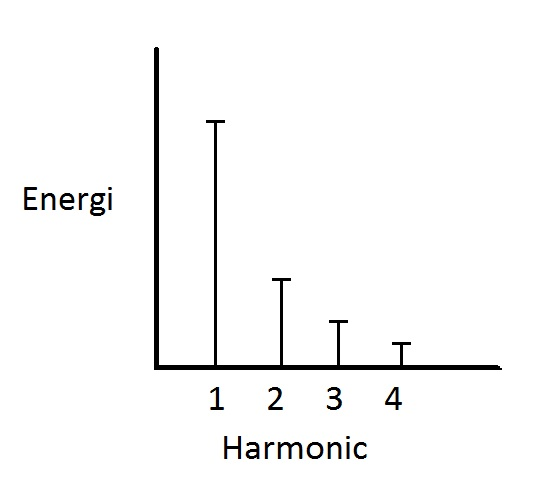
\includegraphics[scale=0.5]{billeder/harmonics}
\caption{n = 4 : harmonics}
\label{fig:harmonics}
\end{figure}
\subsection{Select distance intervals equal to notes}
The idea would be to set intervals for distance much like the distance between keys on a piano. This is shown on figure~\ref{fig:pianokeys}. The idea would then be that you would place a person or an item in the interval and then play a tone with a fixed rate. The rates would then be configurable with buttons on the blackfin for instance.
\begin{figure}[hbpt]
\centering
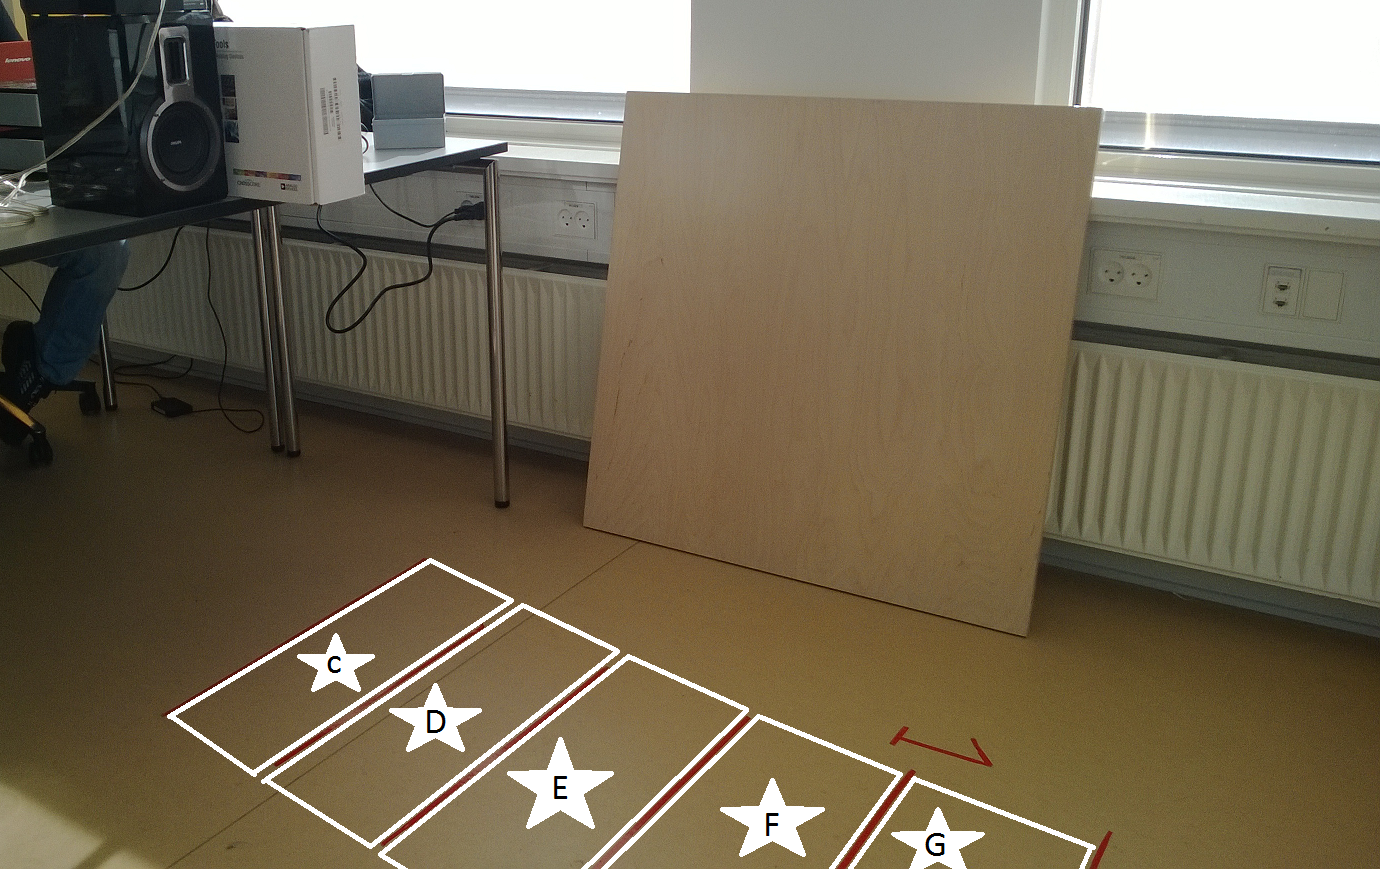
\includegraphics[scale=0.3]{billeder/pianokeyground}
\caption{Piano Keys drawn in front of the system}
\label{fig:pianokeys}
\end{figure}
\section{Buffers sizes}
Noget med størrelsen kan optimeres